\section{PoE SNMP Monitoring Tool}
\label{sec:tool}

\subsection{Architektur}

Das PoE-Tool besteht aus 2 Komponenten.

\begin{description}
  \item [\textbf{Backend}] Die Backend-Komponente erzeugt kontinuierlich
  Messungen für alle definierten Switches durch. Die Zeitintervalle zwischen den Messungen
  werden mittels config-file angegeben. Die Messungen werden weiters in der
  Datenbank abgelegt. Zusätzlich bietet das Backend eine Schnittstelle an welche
  es erlaubt Abfragen auf die gesammelten Measurements zu machen.
  \item [\textbf{GUI}] Die GUI-Komponente nimmt Benutzeranfragen entgegen und
  fragt die darzustellenden Daten vom Backend ab. Das Backend liefert jedoch nur
  Messungen. Die Gruppierung und Konvertierung der Daten in ein übersichtliches
  von Menschen verwertbares Datenmaterial wird ebenfalls von der GUI
  durchgeführt.  
\end{description}


\begin{figure}[h]
    \centering
    \leavevmode
    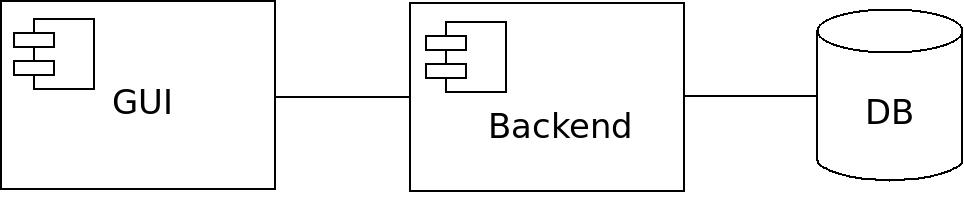
\includegraphics[width=1.0\linewidth]{figures/architecture.jpeg}
    \caption{Software-Architektur PoE}
    \label{fig:Software-Architektue PoE}
\end{figure}

\subsection{Konfiguration}

Das PoE-Tool wird über die Konfigurationsdatei
\textbf{config.properties} angepasst. Diese enthält folgende Optionen:

\begin{description}
  \item [\textbf{measurement.interval}] Dieser Wert gibt die Zeit die zwischen
  Messungen verstreicht in ms an.
  \item [\textbf{distribution.slots}] Dieser Wert gibt in wieviele Zeitslots ein
  Messintervall unterteilt werden soll, um eine gleichmäßigere Verteilung an
  SNMP-Anfragen an die einzelnen Switches zu ermöglichen.
  \item [\textbf{data.retriever.impl}] Dieser Wert gibt an welche Datenquelle
  für die GUI verwendet werden soll. Es gibt 2 Datenquellen. Einerseits eine
  Test-Datenquelle für die GUI
  \textit{cn.poe.group1.collector.DummyDataRetriever} und zusätzlich die
  Datenquelle welche die tatsächlichen Nutzdaten liefert \textit{cn.poe.group1.collector.DataRetrieve}
\end{description}

\subsection{Verwendung}

Durch das Starten des PoE-Tool beginnt dieses automatisch Messungen für alle
definierten Switches zu erzeugen. Durch Auswahl eines entsprechendes Switches in
der linken Tabelle  können für diesen die Nutzdaten angezeigt werden.

\subsubsection{Switch}

Durch Auswahl eines Switches in der linken Tabelle erhält man einen Überblick
über den Switch. Auf der Registerkarte Switch im rechten Teil des Fensters
erhält man einen Überblick den zeitlichen Verlauf der Messungen am Switch.

\begin{figure}[h]
    \centering
    \leavevmode
    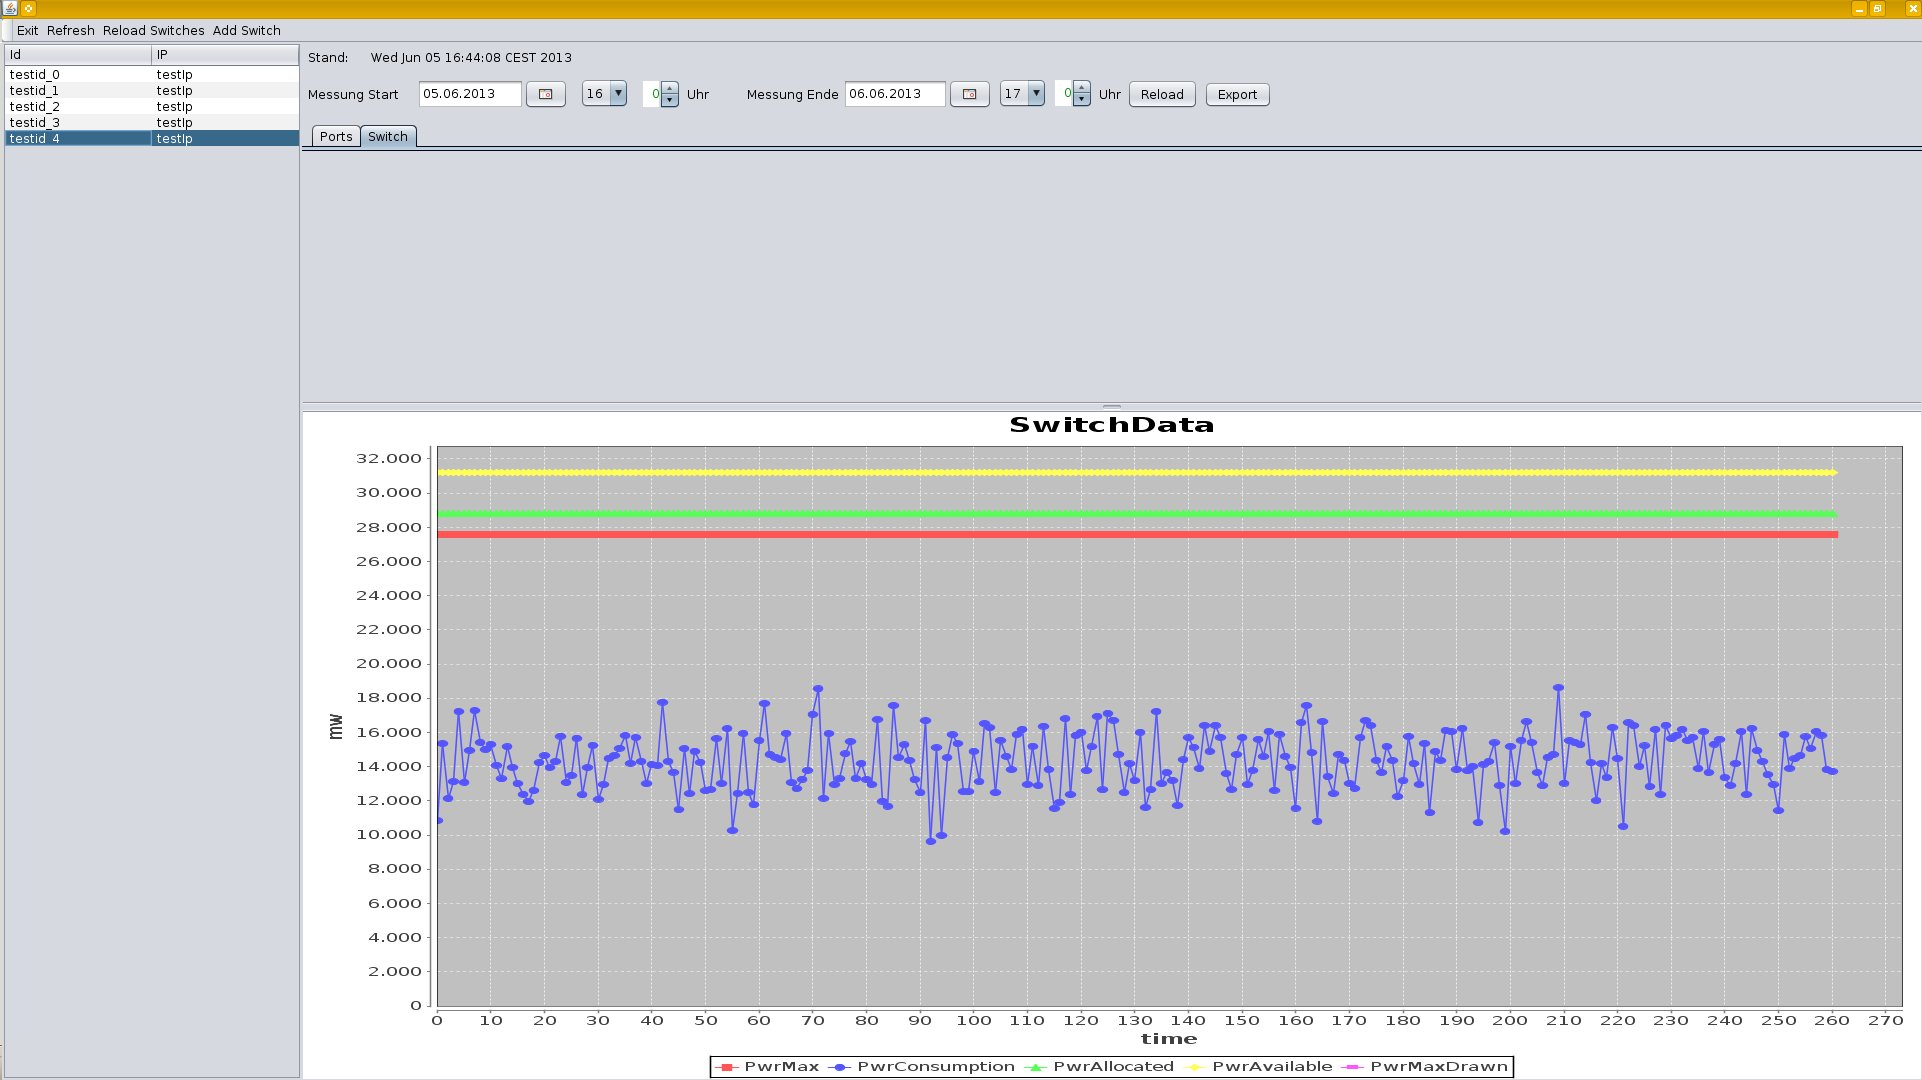
\includegraphics[width=1.0\linewidth]{figures/screenshot2.jpg}
    \caption{Software-Architektur PoE}
    \label{fig:Ports-PoE}
\end{figure}

Durch einen Klick auf \textbf{Add Switch} in der Menüzeile kann man einen neuen
Switch definieren welcher überwacht werden soll. Dazu müssen lediglich die Daten
im Popup ausgefüllt und bestätigt werden.

 \begin{figure}[h]
    \centering
    \leavevmode
    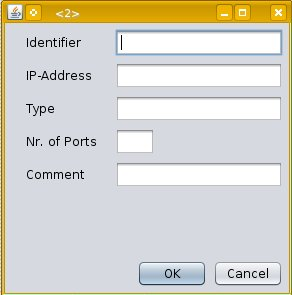
\includegraphics[scale=0.5]{figures/screenshot3.jpg}
    \caption{Software-Architektur PoE}
    \label{fig:NeuerSwitch-PoE}
\end{figure}

\subsubsection{Ports}

Auf der Registerkarte Port im rechten Teil des Fensters

\begin{figure}[h]
    \centering
    \leavevmode
    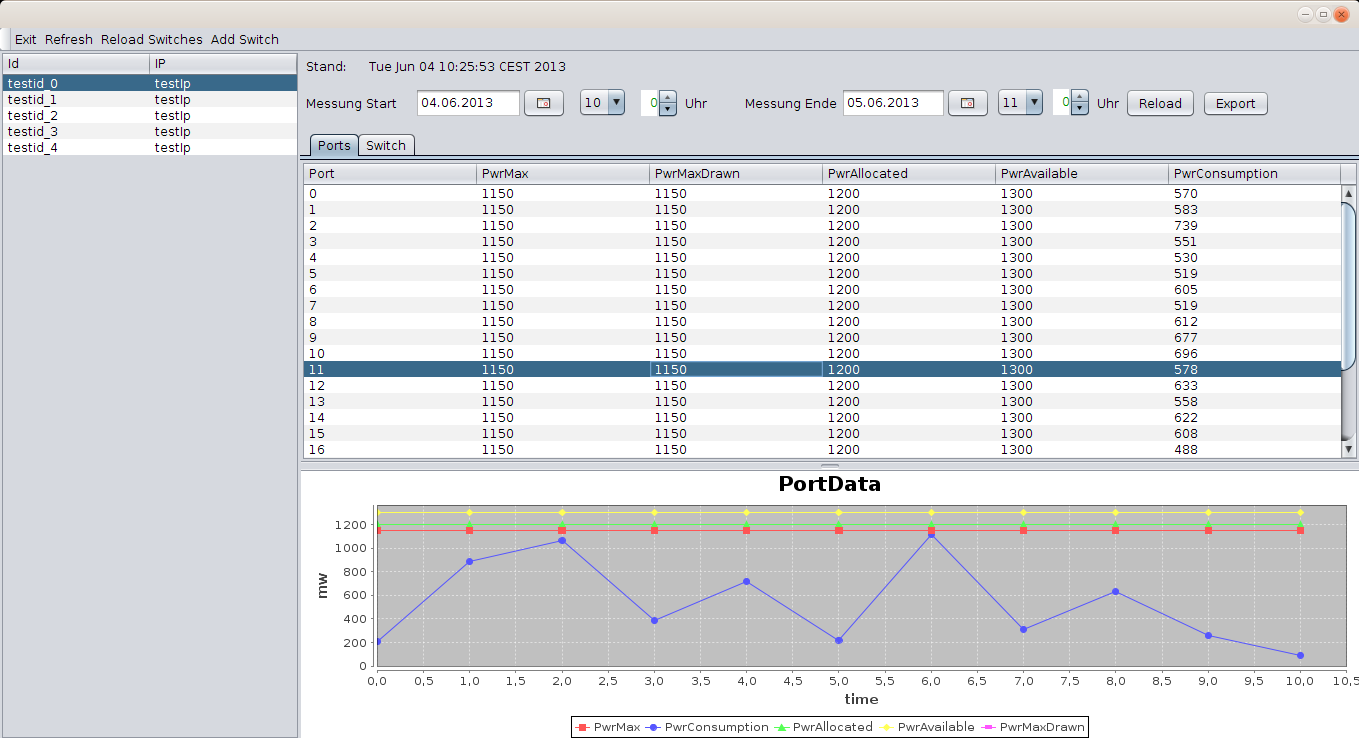
\includegraphics[width=1.0\linewidth]{figures/screenshot1.png}
    \caption{Ports PoE}
    \label{fig:Ports-PoE}
\end{figure}

\subsubsection{Messungen}

\subsubsection{CSV Export}
